\documentclass[manuscript,screen,nonacm]{acmart}
\usepackage{amsmath,booktabs,tabularx,tikz}
\usetikzlibrary{arrows.meta,positioning}
\settopmatter{printacmref=false}
\setcitestyle{numbers,sort&compress}
\setcopyright{none}
\setlength{\emergencystretch}{3em}
\title{When Confidence Exceeds Capacity: A Bounded Study of Intrusion-Detection Triage under Telemetry and Domain Shift}
\author{Ezekiel Ologunde}
\affiliation[obeypunctuation=true]{\institution{Independent Researcher}\country{}}
\email{ologunde@bu.edu}
\authorsaddresses{Author's address: Ezekiel Ologunde, Independent Researcher; email: \href{mailto:ologunde@bu.edu}{ologunde@bu.edu}.}
\begin{document}
\begin{abstract}
Uncertainty-based routing can reduce the number of predictions accepted without review, but a threshold calibrated on one traffic distribution does not impose a capacity limit after deployment. We examine that distinction in a bounded offline study using three official NetFlow-v3 datasets, chronological partitions, conventional classifiers, and simulated loss of feature families. A protocol fixed before model evaluation compares frozen uncertainty thresholds, hourly capacity-constrained uncertainty ranking, and random review at three nominal budgets. We analyze unique predictor patterns sampled from public testbed traffic and retain per-flow predictions for recounting. %ABSTRACT_RESULTS%
The contribution is an auditable characterization of failure conditions, not a new detector or a claim of operational effectiveness. Duplicate removal, conflicting labels under the chosen representation, retrospective batching, and limited domain diversity materially constrain interpretation.
\end{abstract}
\keywords{intrusion detection, selective prediction, domain shift, missing telemetry, review capacity, reproducibility}
\maketitle

\section{Introduction}
An intrusion detector can be uncertain for several reasons: its training network may differ from the observed network, informative fields may be absent, or the available representation may not distinguish benign and attack records. Routing uncertain predictions for additional inspection is a reasonable response, but it creates a separate decision problem. A detector may be calibrated to route five percent of source observations while forwarding a very different fraction after a distribution change. Alternatively, enforcing a strict capacity limit can leave uncertain and incorrect decisions unreviewed. Predictive reliability and review feasibility are therefore distinct outcomes.

This paper examines that distinction using an intentionally conventional learning pipeline. We compare a clean-source calibration threshold with a hard hourly review cap under both domain transfer and feature-family outages. Neither threshold rejection, uncertainty ranking, nor masking is introduced as a new algorithm. The aim is to expose when the operational interpretation of a calibration budget fails, using a reproducible experiment whose limitations can be inspected alongside its results.

The study addresses three questions. RQ1 asks how often a frozen source-calibrated threshold exceeds its nominal review fraction on held-out traffic. RQ2 asks how a strict hourly cap changes unreviewed errors relative to that threshold and random routing. RQ3 asks whether the descriptive outcomes depend on the feature outage, source-target pair, classifier, and mask augmentation. RQ1 and the five-percent threshold-versus-cap comparison are primary; remaining budgets and model comparisons are secondary. A separate representation audit is exploratory and is not used to tune the primary experiment.

Our contribution is the combination of an explicit review-budget estimand, controlled joint-shift comparisons, exact data provenance, and inspectable prediction evidence. The novelty claim is deliberately bounded. The literature already covers budget-aware cross-domain detection and corruption-aware IDS training. This study is an empirical diagnostic of specified conditions and does not establish that all intersections of these areas are unexplored.

\section{Related Work and Contribution Boundary}
RiskGate-IDS studies budget-aware two-stage NetFlow detection across datasets, including target-domain calibration\cite{riskgate}. It directly overlaps the broad motivation for budgeted transfer. Our source-only calibration regime is different from a target-labeled regime, but that difference is an experimental condition rather than sufficient evidence of a new method. Full publisher text could not be retrieved during this study, and the advertised implementation repository returned an unavailable response. We consequently do not claim to reproduce or outperform RiskGate-IDS.

MaskAug reports random masking, block masking, and noise augmentation for intrusion detection\cite{maskaug}. Its accessible abstract includes a matched clean-replication control. Our simpler family-mask variant is an established-method baseline, not an exact MaskAug implementation. Because our variant adds training rows and changes effective forest leaf support, its comparison does not isolate masking from every training-budget effect.

Selective prediction under domain shift is established beyond security. Kamath et al. study confidence and learned error selection for question answering\cite{selective}. This supports treating rejection quality separately from ordinary classification accuracy; it does not imply that a particular selector transfers reliably to network flows. The present study uses uncertainty scores without a learned error selector to keep the primary comparison interpretable.

The NetFlow-v3 release supplies temporal fields and a common extraction framework across several benchmark datasets\cite{temporal}. We use its official archives, not superficially aligned columns from incompatible raw datasets. Common headers do not establish common operational distributions, semantic equivalence of attack families, or contemporary deployment realism. Related-work screening is targeted, not a systematic review. Restricted access to close methods remains a limitation on positioning and should be resolved before making stronger comparative claims.

\section{Data and Integrity Audit}
We obtained NF-UNSW-NB15-v3, NF-ToN-IoT-v3, and NF-CICIDS2018-v3 through the University of Queensland catalogue\cite{catalogue}. Each archive was checked against its supplied payload SHA-1 manifest; additional archive SHA-256 hashes are retained. These checks establish byte consistency with downloaded receipts, not adversarial authenticity or independent label validation. All observed start/end intervals were ordered and nonmissing in the initial audit. UNSW contained 63,425 missing values in SRC\_TO\_DST\_SECOND\_BYTES. Thus, ``clean'' means no added corruption, not universally complete telemetry.

%DATA_TABLE%

The UNSW archive contains 127,693 attack flows, whereas the catalogue lists 127,639. The full row total and benign count agree. We report the downloaded labels and preserve the discrepancy instead of silently substituting the catalogue count. This observation alone does not identify mislabeled individual records. The accompanying feature dictionary also repeats descriptions for several direction-specific fields. We exclude the ambiguous DURATION\_IN and DURATION\_OUT variables from primary prediction rather than assert an unverified interpretation.

Each domain contributes a uniform priority sample of 100,000 flows. A fixed pseudorandom stream assigns a priority to every row; the smallest priorities are retained across the entire archive without consulting labels. This bounded sample makes the experiment feasible locally and must not be described as full-dataset model training. The raw files cover approximately fifty million flows, but experimental independence is governed by domains and captures, not that row total.

\section{Protocol and Methods}
\subsection{Temporal Partitioning and Representation}
We sort the sampled records by flow start time and original row index. The time values at the 60th and 80th sample percentiles define train, calibration, and test boundaries. Training records must end before the first boundary; calibration records must start after or at the first and end before the second; test records start after or at the second. Boundary-crossing records are purged. Equal timestamps remain on one side. Both training and calibration must contain both binary classes or the source fit aborts.

Predictors exclude addresses, absolute timestamps, row identifiers, labels, attack names, DNS transaction IDs, raw ports, layer-7 protocol identifiers, and the two ambiguous duration fields. The remaining numeric IP protocol field is treated as numeric, a pragmatic baseline choice rather than an optimal encoding. This service-reduced representation limits some environment-specific shortcuts but may also remove genuine distinguishing information.

We remove duplicate complete predictor vectors within partitions and exclude calibration/test vectors already present in earlier source partitions. Across-domain tests additionally exclude predictor vectors present in source training or calibration. The earliest retained occurrence determines the label of a repeated pattern. Hash-based matching uses a fixed pandas representation; cryptographic or collision-free identity is not claimed. This procedure targets previously unseen unique patterns. It changes prevalence and does not estimate traffic-volume accuracy. The implications of conflicting labels are examined explicitly below.

%SPLIT_TABLE%

\subsection{Models and Controlled Missingness}
We use logistic regression with regularization parameter $C=1$ and a 500-iteration limit, and a random forest with 100 trees, maximum depth 16, and minimum leaf size five. Seeds are 17, 29, and 43. We perform no test-directed hyperparameter search, class reweighting, or attack oversampling. Missing values receive source-training medians and explicit indicators for every field. Signed log transformation and source-trained standardization are applied through a common preprocessing function for both classifiers. Forest splits depend primarily on order, but finite precision prevents a claim of exact equivalence to untransformed fitting.

Complete-data training is compared with adding one masked copy of each training row. The copy has one uniformly selected temporal, size, or TCP family hidden. Original source medians are retained; scaling is fitted to the actual training variant. The temporal family contains inter-arrival and flow-duration fields; size includes byte, packet, length, and throughput fields; TCP includes flag and window fields. Their exact membership is saved with the split receipt and disjointness is asserted.

Evaluation conditions are no additional corruption, temporal outage, size outage, TCP outage, temporal-plus-TCP outage, and ten-percent independent cell masking. A family outage applies to every evaluated flow. It represents fields absent from an exporter schema, not packet loss. Inferring packet-loss effects would require recomputing features from packets. Random masks are seeded and shared by paired comparisons. Source calibration always uses the uncorrupted condition, deliberately testing a frozen policy when telemetry changes.

\begin{figure}[t]
\centering
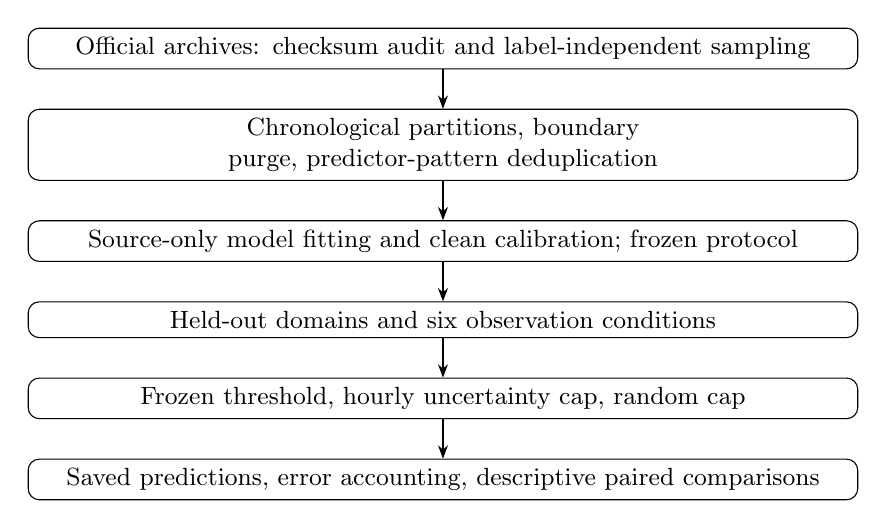
\begin{tikzpicture}[node distance=5mm, every node/.style={draw,rounded corners,align=center,font=\small,text width=10.3cm}, >=Stealth]
\node (a) {Official archives: checksum audit and label-independent sampling};
\node (b) [below=of a] {Chronological partitions, boundary purge, predictor-pattern deduplication};
\node (c) [below=of b] {Source-only model fitting and clean calibration; frozen protocol};
\node (d) [below=of c] {Held-out domains and six observation conditions};
\node (e) [below=of d] {Frozen threshold, hourly uncertainty cap, random cap};
\node (f) [below=of e] {Saved predictions, error accounting, descriptive paired comparisons};
\draw[->] (a)--(b);\draw[->] (b)--(c);\draw[->] (c)--(d);\draw[->] (d)--(e);\draw[->] (e)--(f);
\end{tikzpicture}
\caption{Experiment workflow. Target labels are used for evaluation only. The representation ambiguity audit is a separate exploratory diagnostic.}
\Description{Six sequential boxes show acquisition, temporal partitioning, source fitting, held-out evaluation, review policies, and prediction verification.}
\end{figure}

\subsection{Review Policies and Metrics}
Let $p_i$ be the predicted attack probability. Classification uses $p_i\geq0.5$, and uncertainty is $u_i=1-|2p_i-1|$. For nominal budget $b\in\{0.01,0.05,0.10\}$, frozen routing reviews a record if $u_i$ exceeds the upper empirical $(1-b)$ calibration quantile. Strict comparison avoids routing all observations tied at the threshold. The budget is a calibration property, not a target guarantee.

Capacity-constrained routing groups evaluated sample records by their UTC start hour and selects the $\lfloor bn_h\rfloor$ highest-uncertainty records in each hour $h$. Original row order breaks ties. Random routing selects the same number using seeded random priorities. These are retrospective hourly policies: scores for the full batch are available before selection. They entail waiting time and do not demonstrate real-time queue stability or analyst throughput in a deployed system.

For review indicator $r_i$, error indicator $e_i$, and $n$ observations, we report
\begin{equation}
R=\frac{\sum_i r_i}{n},\qquad E_U=\frac{\sum_i(1-r_i)e_i}{n},\qquad E_A=\frac{\sum_i(1-r_i)e_i}{\sum_i(1-r_i)}.
\end{equation}
$R$ is review fraction, $E_U$ unreviewed error per input, and $E_A$ accepted risk. Undefined denominators remain undefined. We also retain false negatives, false positives, error capture, attack-family counts, and hourly aggregates. Routing an error is not equivalent to correcting it: no human-review accuracy or attack-prevention benefit is assumed.

\subsection{Analysis and Reproducibility}
Six ordered cross-domain pairs are primary; three within-domain comparisons are diagnostics. Seeds measure algorithm variability and do not create new network domains. Tables use descriptive equal-cell means where indicated; these are not estimates of pooled operational prevalence. We report directional paired comparisons without flow-independent significance tests. No confidence interval is used to imply that correlated records constitute independent trials.

The protocol and implementation were committed before model outcomes. The first execution failed after its UNSW-source fits because pandas returned a read-only array. An explicit copy repaired the compatibility error without changing the scientific settings. Partial results and logs are retained separately from the complete restart. This is a repeated execution, not a second independent replication. A separate verifier recounts saved prediction errors and frozen routing, checks conservation identities, and checks hourly capacity counts without importing evaluator functions. It does not independently validate labels, sample construction, or model fitting.

\section{Results}
%RESULTS_TEXT%

%CONDITION_TABLE%

%PAIR_TABLE%

\begin{figure}[t]
\centering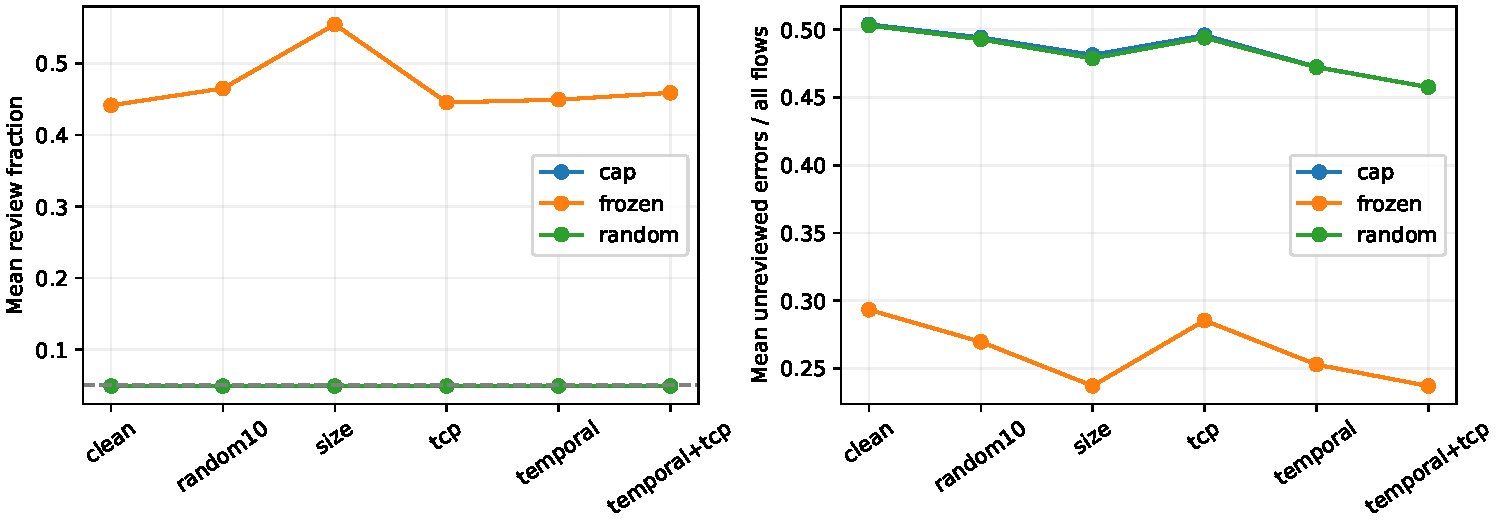
\includegraphics[width=\linewidth]{conditions.pdf}
\caption{Descriptive means over cross-domain model, training, and seed cells at a five-percent nominal budget. Left: actual review fraction. Right: errors remaining outside review per input. The dashed line marks the nominal fraction. Cells reuse data and are not independent replications.}
\Description{Two panels compare frozen-threshold, capacity-constrained and random review across six telemetry conditions.}
\end{figure}

\section{Representation Ambiguity: An Exploratory Diagnostic}
After the protocol was frozen, we audited label conflicts among identical predictor vectors in each full sample. For pattern $x$, let $n_0(x)$ and $n_1(x)$ count its two labels. Any deterministic classifier restricted to this representation incurs at least $\sum_x\min\{n_0(x),n_1(x)\}$ errors on that fixed multiset. This is a finite-sample information bound, not a held-out or deployment guarantee. It uses all sample labels and is never used to choose the primary model or features.

%AMBIGUITY_TABLE%

Reintroducing the excluded service identifiers and duration fields substantially reduces the empirical ambiguity in two domains. This does not identify which individual field is responsible, establish that the additional features transfer safely, or validate ambiguous feature descriptions. It demonstrates a tension: removing shortcuts can also remove information needed to distinguish labeled records. Deduplication further changes the evaluation by selecting one observed label for each repeated pattern and excluding previously seen patterns. A review-budget result under that protocol must not be presented as volume-weighted detection effectiveness.

\section{Discussion and Threats to Validity}
The central design lesson is to state what a budget constrains. A calibration quantile constrains review on its calibration sample. A hard batch cap constrains routing volume on the evaluated batch. Neither construction alone ensures low accepted error, recovery of rare attacks, accurate human adjudication, or sustainable SOC operations. A threshold may appear beneficial because it spends substantially more review capacity. Conversely, a cap can satisfy capacity while leaving many incorrect predictions untouched. Comparing error rates without realized review rates obscures that tradeoff.

The domain set is small and derives from historical controlled traffic. Cross-domain transfer is not a substitute for prospective deployment validation. Attacks occurring late in a capture may differ from those available for training; binary labels combine distinct mechanisms. We preserve time separation but do not claim to isolate covariate shift from label, prevalence, or concept changes. Different capture dates are not randomized treatments.

Representation choices and duplicate removal are especially consequential here. We intentionally measure unique patterns after source overlap removal. This prevents some obvious repeated-pattern leakage, but changes class balance, removes ambiguous occurrences, and can yield a target sample that depends on the source. Tables retain pair-specific denominators for that reason. The exploratory ambiguity audit demonstrates that these constraints are material, not merely generic caveats. The retained earliest label is not independently adjudicated ground truth for the pattern.

Our missingness manipulations are controlled feature omissions, not empirical sensor failures. Natural missingness already exists in one source. Corruption at training and testing may differ, and a mask indicator can itself become a domain cue. Source-only imputation and scaling prevent target-label tuning but do not remove all representation shift. The augmentation comparison is secondary and lacks a matched repeated-clean training control; it cannot establish a uniquely causal masking benefit.

Uncertainty from class probabilities is only one possible review score. Error predictors, class-specific costs, target calibration, and queue-aware online policies may change the conclusions. We omit them from the frozen study rather than select additions after inspecting results. Review capacity is measured as a fraction of sampled unique patterns, not minutes of analyst time or the full traffic arrival process. Hourly flooring can yield slightly less review than the nominal percentage and assigns zero slots to sufficiently small batches. No correction accuracy is attributed to a human or second-stage detector.

The study supports a bounded evaluation contribution. Close work already covers broad components, and inaccessible full texts limit a definitive novelty judgment. The absence of an exact matched implementation comparison means the results cannot support state-of-the-art superiority. A subsequent extension should use a separately frozen protocol with volume-weighted evaluation, a matched augmentation control, independent label assessment where possible, and a prospective or additional-domain test set. More compute alone would not resolve these scientific limitations.

\section{Conclusion}
This study separates source-calibrated uncertainty routing from an enforced review limit and measures both under controlled telemetry and domain changes. The results quantify realized review, residual errors, and dependence on the chosen evaluation representation. The released protocol, audit receipts, partial-failure record, aggregate results, and prediction hashes make those boundaries inspectable. The study does not establish a new IDS algorithm, operational SOC benefit, or exclusive novelty. Its practical recommendation is to report achieved capacity and remaining errors together, while making sampling, duplicate handling, and feature information loss explicit.

\section*{Data, Code, and Author Statement}
Code, protocols, aggregate results and build materials are available at \url{https://github.com/ezekielologunde/ids-telemetry-shift}. Raw public archives and locally generated sample/prediction artifacts remain outside Git; acquisition links, hashes and regeneration commands are supplied. The official dataset pages specify permitted reuse with a commercial-use restriction. Original project work remains unlicensed at the author's direction; third-party terms continue to apply. No live third-party systems, private operational telemetry, human subjects, or paid model APIs were used. All fitting for this bounded study ran locally; no ASA-X execution is claimed. This is an ACM-class research manuscript for author review, not an accepted paper or a record of journal submission.

\begin{thebibliography}{9}
\bibitem{riskgate} Budget-aware two-stage NetFlow intrusion detection for high-traffic critical information infrastructure under domain shift. 2026. Publisher record, PII S187454822600048X. \url{https://www.sciencedirect.com/science/article/abs/pii/S187454822600048X}. Accessible indexed abstract and sections consulted; full methods unavailable.
\bibitem{maskaug} Qianli Di, Keju Du, Gang Chen, and Hai Deng. 2026. MaskAug: Architecture-agnostic corruption-aware training for robust network intrusion detection. \emph{Journal of Computer Security}, OnlineFirst. \url{https://doi.org/10.1177/0926227X261487917}. Accessible abstract consulted.
\bibitem{selective} Amita Kamath, Robin Jia, and Percy Liang. 2020. Selective Question Answering under Domain Shift. In \emph{Proceedings of ACL}, 5684--5696. \url{https://doi.org/10.18653/v1/2020.acl-main.503}.
\bibitem{temporal} Majed Luay, Siamak Layeghy, Seyedehfaezeh Hosseininoorbin, Mohanad Sarhan, Nour Moustafa, and Marius Portmann. 2026. Temporal Analysis of NetFlow Datasets for Network Intrusion Detection Systems. arXiv:2503.04404v3. \url{https://arxiv.org/abs/2503.04404v3}.
\bibitem{catalogue} University of Queensland. Machine Learning-Based NIDS Datasets. Accessed 7 October 2026. \url{https://staff.itee.uq.edu.au/marius/NIDS_datasets/}.
\end{thebibliography}
\end{document}

